
\begin{figure}
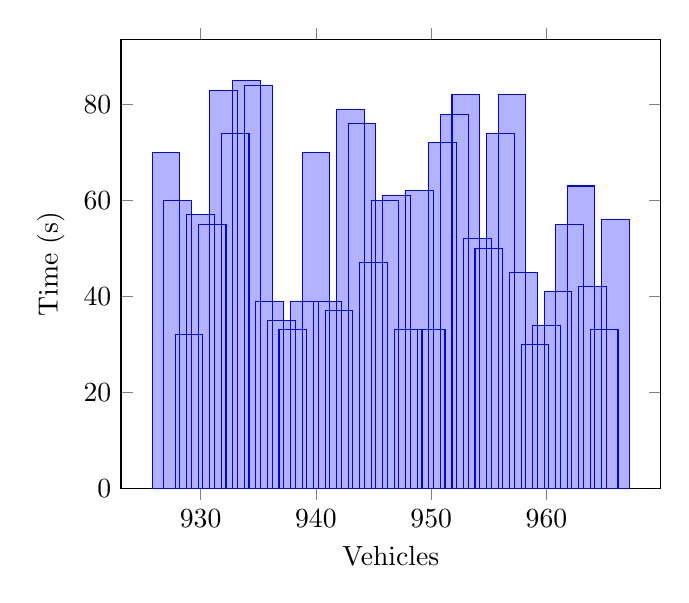
\begin{tikzpicture}
\begin{axis}[
legend style={anchor=west},
xlabel=Vehicles,
ylabel=Time (s),
ymin=0,
ybar,
]
\addplot coordinates {
(951, 72)
(948, 33)
(949, 62)
(946, 60)
(947, 61)
(944, 76)
(945, 47)
(942, 37)
(943, 79)
(940, 70)
(941, 39)
(927, 70)
(938, 33)
(933, 74)
(932, 83)
(931, 55)
(930, 57)
(937, 35)
(935, 84)
(934, 85)
(928, 60)
(929, 32)
(952, 78)
(939, 39)
(964, 42)
(965, 33)
(966, 56)
(960, 34)
(961, 41)
(962, 55)
(963, 63)
(936, 39)
(956, 74)
(953, 82)
(959, 30)
(958, 45)
(950, 33)
(955, 50)
(954, 52)
(957, 82)
};

\end{axis}
\end{tikzpicture}
\label{tik:time:0:13}
\caption{0 percent diving with GSC on route $13$}
\end{figure}
